\section{Experiments}\label{sec:experiments}

In this section, we report on experimental measurements illustrating the concrete improvements
in latency of PoEM as compared to Bitcoin. We implemented a stochastic simulation in 1500 lines of
Rust code\footnote{%
    The source code will be made available in the full version of this paper. % TODO
    \ifanonymous
        % TODO
    \else
    \fi
} to compare the two protocols.

% \subsection{Experimental Methodology}\label{sec:methodology}
%
% We ran multiple simulations\footnote{
%     The source code resides in the following \ifanonymous anonymized \fi repositories:
%     \ifanonymous
%     \begin{enumerate}
%         \item \url{https://anonymous.4open.science/r/go-quai-228B}
%         \item \url{https://anonymous.4open.science/r/go-quai-3FB2}
%         \item \url{https://anonymous.4open.science/r/go-quai-8610}
%         \item \url{https://anonymous.4open.science/r/go-quai-DCB6}
%         \item \url{https://anonymous.4open.science/r/simulation-0549}
%         \item \url{https://anonymous.4open.science/r/quai-cpu-miner-7065}
%     \end{enumerate}
%     \else
%     \begin{enumerate}
%         \item \url{https://github.com/gameofpointers/go-quai/tree/poem-sim-honest}
%         \item \url{https://github.com/gameofpointers/go-quai/tree/bitcoin-sim-honest}
%         \item \url{https://github.com/gameofpointers/go-quai/tree/poem-sim-adv}
%         \item \url{https://github.com/gameofpointers/quai-cpu-miner/tree/sim-miner}
%         \item \url{https://github.com/gameofpointers/simulation}
%     \end{enumerate}
%     \fi
% }
% in order to ascertain the optimal configuration for
% operating both Bitcoin and PoEM in order to achieve the minimum confirmation delay.
% We simulated an artificial network delay of $\Delta$ (measured in seconds) in the
% communication between the honest parties in order to indirectly control the honest
% block production rate $g$, measured in blocks per network delay. We define $g$ to
% be the number of valid blocks cumulatively produced by the honest parties in one
% network delay on average, including blocks that were subsequently abandoned
% (following the terminology in~\cite{eiar}). This corresponds to the average number of
% successful honest random oracle queries per network delay.
% In the meantime,
% we kept the mining target $T$ constant throughout the simulations (instead of varying
% the network delay $\Delta$ and keeping $T$ constant, we could have, equivalently, kept
% $\Delta$ constant and varied the target $T$). The target $T$ was not dynamically adjusted
% during the simulation, in order to mimic the static nature corresponding to our theoretical
% analysis.
% Our goal was to plot the confirmation delay $d$ (in units of the network delay $\Delta$)
% as a function of the block production rate $g$ for both systems.
%
% All executions included exactly
% $n = 49$ parties, of which $t = 12$ were adversarial and $n - t = 37$ were honest.
% The adversarial ratio was $\beta = \frac{t}{n} = 0.244$.
% The honest parties ran the honest code of Bitcoin or PoEM respectively.
% We fixed the adversarial strategy to be the private mining attack, which was
% proven~\cite{eiar} to be the best possible attack against Bitcoin in the
% continuous-time domain~\cite{bitcoin-made-simple}. This means that the network
% began with a genesis block given to all honest and adversarial parties. The adversary
% then mined blocks in private on her own chain, whereas the honest parties mined
% their own blocktree without intervention by the adversary, following the heaviest chain
% rule (in Bitcoin) or the most intrinsic work rule (in PoEM) respectively. To emulate the puppetmaster
% nature of the adversary, we imposed no artificial network delay for the adversary.
% On the contrary, every honest message was artificially delayed by exactly the maximum
% delay bound $\Delta$.
%
% Simulations were run on 49 virtual machines in Google Cloud all co-located in
% the same data center. The configuration of the nodes used was 4 CPU cores, 4
% GB of RAM, with a 10 GB SSD running Ubuntu 22.4. The honest party
% had an artificial network delay between 100-1000ms (to allow for simulating varying
% $g$). This delay was achieved by adding a \texttt{sleep} prior to every block message
% broadcast. The adversary's network delay was only the inherent delay in communication
% between virtual machines and was <5 ms. The tests were coordinated using Ansible and the
% machines were given 2 minutes to peer with each other and stabilize at the beginning of
% each test.
% Both Bitcoin and PoEM were run on the same codebase,
% with the exception of the appropriate modification to the proof-of-work inequality.
%
% We ran each simulation until one of the honest parties managed to obtain a chain of
% length $200$ blocks, at which point the simulation was halted and its lifetime $L$
% (in units of $\Delta$) was measured. We recorded $g$ for that simulation as the number
% of honest blocks produced divided by $L$ to find the average number of honest blocks
% produced per network delay (regardless of whether they were ultimately abandoned or not).
%
% For Bitcoin, at every block height
% $1, \ldots, 200$ that appeared in the simulation, we recorded a flag indicating whether
% the first party to mine at this height was honest or adversarial. For each configuration of $g$, we
% repeated the simulation $100$ times in a Monte Carlo fashion, and chose the value
% $k^*$ to be the block height such that at least $90\%$ of the Monte Carlo simulations
% indicated that, within that simulation, the honest parties were ahead of the adversary from height $k^*$
% onwards. This corresponds to accepting a probability of Common Prefix failure of
% up to $10\%$.
% We calculated the average honest chain growth rate $f$ as $f = L / 200$
% (noting that $f \leq g$ and $0 \leq f \leq 1$, roughly following the terminology
% of the Analysis section, and observing that, due to the heaviest chain rule,
% the chain can grow no more than $1$ block per network delay when the honest
% parties are operating alone).
% The confirmation delay ($d$) for each configuration $g$ was obtained by dividing
% this $k^*$ by $f$ to calculate the time (in units of network delay $\Delta$)
% needed to get $k^*$ blocks on average.
%
% In PoEM's case, we mark the cummulative chain work at every $\work$ point in intervals of $\gamma + \frac{1}{\ln2}$
% (corresponding to the expected amount of work per valid block),
% namely $\gamma + \frac{1}{\ln2}, 2\left(\gamma + \frac{1}{\ln2}\right),\allowbreak\ldots,\allowbreak 200\left(\gamma + \frac{1}{\ln2}\right)$.
% For each of those $\work$ points, we record a flag indicating whether the honest
% parties or the adversary first mined a chain with at least that amount of work.
% Similar to the Bitcoin experiments, we ran $100$ Monte Carlo simulations and
% calculated $k^*$ to be the $\work$ point such that at least $90\%$ of the
% Monte Carlo simulations indicated that, in this simulation, the honest parties were ahead of the
% adversary from that $\work$ point onwards. The confirmation delay ($d$) for
% each configuration $g$ was obtained by dividing this $k^*$ by $\frac{f}{\gamma + \frac{1}{\ln2}}$
% to calculate the time needed to get $k^*$ work on average.
%
% \subsection{Experimental Results}\label{sec:results}
%
% Figure~\ref{fig:results}(a) illustrates the evolution of $d$ across different $g$ values. We
% identified the best operating conditions for a protocol as the point where the
% confirmation delay is minimized. In our simulations, Bitcoin achieved its lowest
% delay of $25.58 \Delta$ at a block rate of $g=0.98$. On the other hand, at the same
% $g$, PoEM reached the minimal delay of $18.29 \Delta$ operating with
% $\gamma=10$. This means for the configuration minimizing the delay of each protocol,
% PoEM had a $\frac{25.58 - 18.29}{25.58} = 28.5\%$ lower confirmation delay as compared to Bitcoin.
%
% When either system operates at higher block production rate $g$, the honest chain
% grows faster ($f$ also increases), but the confirmation delay $d$ increases as well.
% We found that the relationships between $g$ and $f$ in Bitcoin and PoEM are
% comparable (Figure~\ref{fig:results}(b)). However, for a given delay, PoEM can
% safely operate at a higher block production rate $g$ than Bitcoin, yielding an
% operation point with a higher honest chain growth rate $f$. In particular, we
% found that, for example at $d = 25.6\Delta$, Bitcoin gives a chain growth rate
% of $f = 0.43$, whereas PoEM, for a close delay of $d = 27.4\Delta$,
% gives a chain growth rate of $f = 0.5$, marking a $16.3\%$ improvement in
% transaction throughput.
% % Specifically, PoEM increases $f$ from 0.43 to 0.5, marking a 16.3\%
% % improvement, for a comparable confirmation delay (Bitcoin($d=25.6$),
% % PoEM($d=27.4$))

We simulate various executions of Bitcoin and PoEM with different parameterizations.
In each execution simulation, we fix the block production rate $g$, the adversarial ratio $\beta$,
and, for PoEM, also the bias parameter $\gamma$, and we
measure the latency of the system. The latency is defined as the time it takes for a new transaction
to become stable in the system (i.e., $k$-confirmed for a sufficiently large $k$).
The challenge is to measure the latency of the two
systems at the same \emph{security level}. As the two systems operate differently, simply
taking the same number of blocks (or work) does not constitute a fair comparison.

We measure the time needed from the moment an honest block is mined until
the first time any honest party considers the block \emph{stable}, and only for those blocks
which eventually do become stable.
We use the private mining attack as the adversarial strategy, which was
proven~\cite{eiar} to be the best possible attack against Bitcoin in the continuous-time model~\cite{bitcoin-made-simple}.
In a nutshell, in this strategy, the adversary mines blocks in private on her own chain, whereas the honest parties mine
their own blocktree, following the heaviest chain rule (in Bitcoin) or the most intrinsic work rule (in PoEM) respectively.
The adversary imposes a network delay of $\Delta$ to honest parties.
Our simulation begins with all honest parties and the adversary agreeing on a particular block
$B$ with no premining having occurred. At that point, the adversary uses the private mining strategy
to conduct a double spend in a block immediately following $B$.
For a particular execution simulation sample, we determine the \emph{safe} confirmation parameter $k$
that the honest parties \emph{should} have used to avoid this double spend.
Whereas in our experiments, this confirmation parameter is determined retroactively,
in the real implementation, the confirmation parameter should be determined prospectively.

We simulate the adversary and the honest parties independently. On the one hand, the adversary mines blocks
in a chain without incurring any delay, and therefore without any forks. The adversary's block production rate is
$g\frac{\beta}{1 - \beta}$. On the other hand, the honest parties incur a network delay of $\Delta$ for each mined block,
and they mine blocks at a rate of $g$. Because of this delay, the blocks mined by the honest parties form a blocktree.

To save time, instead of wastefully simulating proof of work, we artificially simulate block production by a
continuous-time stochastic process.
We know that the time between the creation of two honest blocks is exponentially distributed
with rate $g$ (because the times of block creation form a Poisson point process~\cite{bitcoin-made-simple}).
Hence, we take multiple independent samples from $\exp(g)$ to get the interval between each successive honest block production event,
thereby giving rise to a Poisson process of honest block creations (even though these blocks may not necessarily be placed in a chain).
We simulate a similar independent Poisson process for the adversary
by sampling from $\exp(g\frac{\beta}{1 - \beta})$. These two stochastic processes produce the block creation times of the honest and
adversary parties, from which we can determine the blocktree that was constructed taking the delay into account.

In Bitcoin, the work of each block is equal to one,
whereas in PoEM, the work of block is exponentially
distributed with rate $\gamma + \frac{1}{\ln2}$ (and note that these exponential samples of \emph{work} are a different,
parallel process from the exponential samples of \emph{time intervals} between block creations).
Hence, in PoEM's case, we sample from $\exp(\frac{1}{\ln2})$ to get the work
of each block in the execution. The creation time of each block and its work are enough to simulate the honest parties' execution
and determine the blocktree that was constructed.
The honest blocktree is computed as follows. We create a list of \emph{events} pertaining to either the creation of a new honest block,
or the arrival of the block to the rest of honest parties $\Delta$ later. We sort these events in chronological order and process them one by one.
Throughout time, we maintain a single value indicating the cumulative work of the heaviest chain seen so far by all honest parties.
For every block, we also keep the cumulative work of the chain ending at that block.
At the block creation event, we compute the cumulative work associated with the block as the cumulative work of the
heaviest chain seen so far plus the work of the block (1 in Bitcoin, sampled in PoEM). At the block arrival event, we compare the
cumulative work of the chain ending at the arrival block with the cumulative work of the heaviest chain seen so far.
If it is heavier, we update our best cumulative work value. Every time we update the best cumulative work value,
we remember this cumulative work together with the creation timestamp associated with the block that cause the work to increase.
% TODO: Cite EiaR for the Δ optimality
% TODO: assume n -> inf

Then, independently we simulate the adversary's execution. Like in the honest execution, we sample from $\exp(g\frac{\beta}{1 - \beta})$
to get the interval between the time of successive adversarially produced blocks, where $g\frac{\beta}{1 - \beta}$ is the adversary's block production rate.
Then, similar to the honest simulation, we set the work of each block to $1$ in Bitcoin, and sample from $\exp(\frac{1}{\ln2})$ to get the work of each block in PoEM.
Since the adversary has no network delay, all her blocks are chained in series.
Again, we maintain an association of timestamps and cumulative work values for every block.
% TODO: Talk about the initial sampling of the adversarial execution and the scaling with $\beta$ retroactively

Having simulated the honest and adversary executions, we can determine the latency of the system (whether this system is Bitcoin or PoEM).
To find this latency, we must find the minimum \emph{safe} confirmation parameter $k$ (where $k$ is denominated in amount of work per block, as measured
by the respective system).
To do this, we determine the \emph{last} point in time when the adversary had a chain with more work than the honest parties,
and we record the work $k$ of the honest chain that first surpasses the adversary's chain immediately after.
For this execution, a confirmation parameter larger or equal to $k$ would safeguard the protocol from a Common Prefix violation.
% TODO: Footnote that this k is safe only against the EiaR attack, and not other possible attacks, even though EiaR is the
% best possible attack wrt resilience.

To accurately calculate the latency of a given system parameterization $(g, \beta)$, we simulate multiple such executions and record the minimum safe confirmation
% TODO: What is your Monte Carlo iteration count?
parameter $k$ for each execution. We collect these $k$ values into a list $K$. We wish to determine the value of $k$ that gives a specific
security level -- in our case, we want $90\%$ of the executions to be safe from a Common Prefix violation (i.e., $3.32$ bits of
security\footnote{While $\lg_2(10\%) = 3.32$ bits of security are not enough for cryptographic security, we use this as a qualitative
reference to compare the latency of the two systems. Our theoretical analysis shows that PoEM is secure with overwhelming probability
in the security parameter $\kappa$.}).
Intuitively, using a common reference security level is what allows us to fairly compare these disparate systems.

In a nutshell, we set $k^*$ to be the minimum confirmation parameter that would safeguard $90\%$ of the executions against a Common Prefix violation.
More precisely, we take the $20\%$ highest percentile of the list $K$ and set $k^*$ to be the mean of these values (i.e., the \emph{expected shortfall}
at $20\%$, noting that the $90\%$ mark falls in the middle of the top $20\%$ percentile).
% TODO: infinite values not taken into account
% TODO: lifetime of simulations

The latency of the system is now calculated as $d = \frac{k^*}{f}$, were $f$ is the average cumulative work increase rate for the honest chains.
Roughly, $d$ measures the average time it takes to produce $k^*$ chained work in the system (both in Bitcoin and PoEM).
% TODO: Explicitly write out what f is

To get the optimal system latency given an adversarial ratio $\beta$, we explore the latency of the system for various block production rates $g$.
The $g$ that minimizes the latency of the system is the optimal block production rate for a given adversarial ratio $\beta$.

% TODO: Quantization
% TODO: Rust code, lines of code, visualization in Python

% TODO: Figures?
% TODO: What about γ?
% TODO: Interpret the plots and tell us a narrative about the results.

% Figure 1:
%   Latency of Bitcoin and PoEM for various parameterizations (horizontal axis is β, vertical axis is latency, optimize over g and γ)

% Figure 2:
%   PoEM executions across different βs (horizontal axis is β, vertical axes are larency, optimal g, optimal γ)
%
% Figure 3:
%   Optimization of γ. Fix (β=0.1, g=0.7) and (β=0.3, g=1.5), vary γ, plot latency. 100k iterations.
%
% Figure 4:
%   Optimization of g. Fix β=0.2, fix γ=0, vary g, plot latency. 100k iterations.

\begin{figure}[pt]
    \centering
    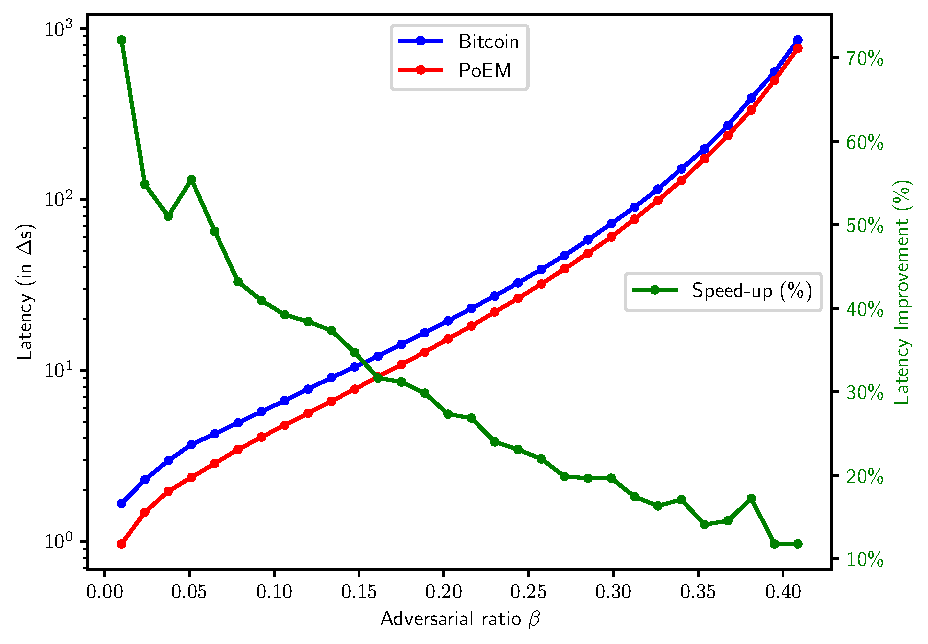
\includegraphics[width = 0.9\textwidth]{figures/bitcoin_vs_poem.pdf}

    \caption{Bitcoin vs PoEM latency over different adversarial ratios $\beta$.
            The results were obtained by running 100k simulations per point.}
    \label{fig:bitcoin_vs_poem}
\end{figure}

\begin{figure}[pt]
    \centering
    \begin{subfigure}{0.48\textwidth}
    \centering
    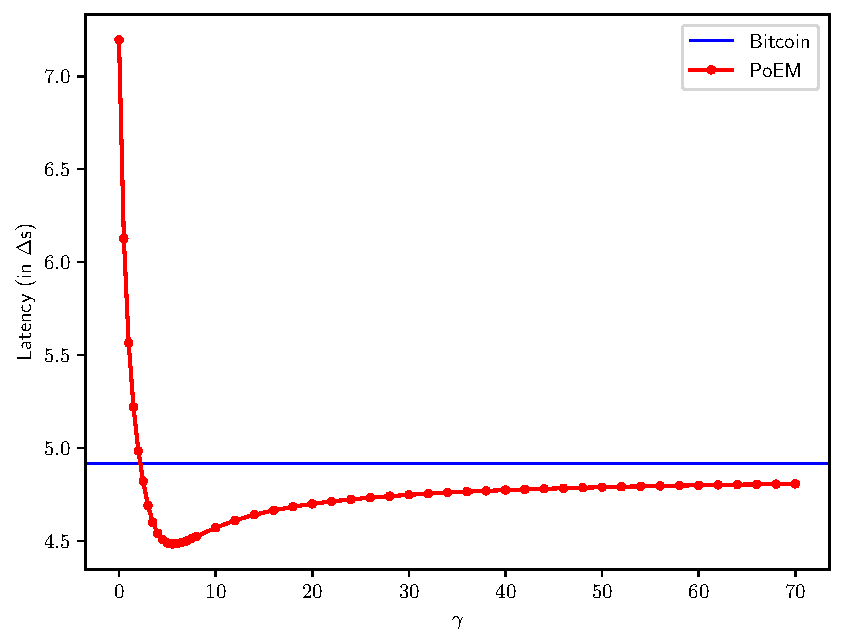
\includegraphics[width = \textwidth]{figures/gamma_latency_0.1.pdf}
    \caption{$\beta = 0.1$ and $g = 0.7$}
    \label{fig:gamma_latency_0.1}
    \end{subfigure}
    \begin{subfigure}{0.48\textwidth}
    \centering
    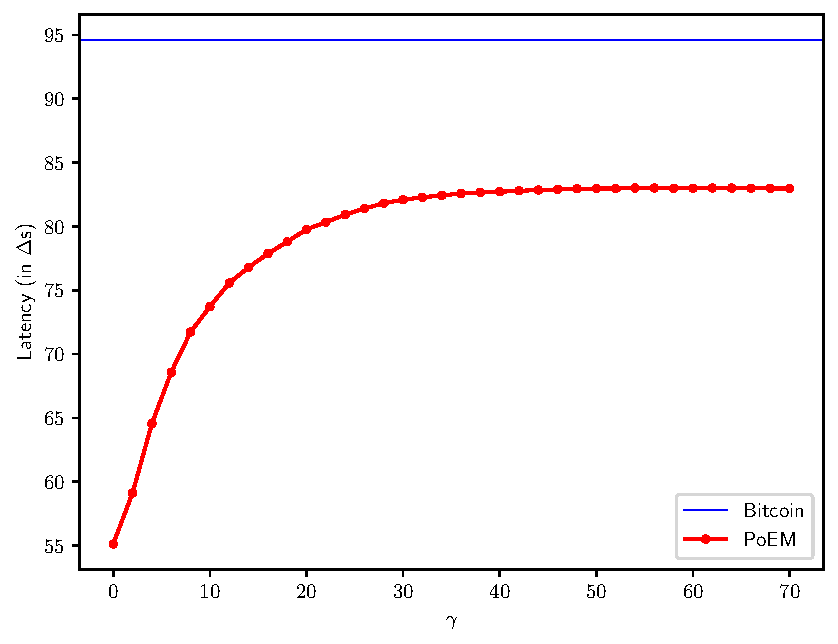
\includegraphics[width = \textwidth]{figures/gamma_latency_0.3.pdf}
    \caption{$\beta = 0.3$ and $g = 0.7$}
    \label{fig:gamma_latency_0.3}
    \end{subfigure}

  \caption{Fixing $\beta$ and $g$, we compare the latency of PoEM parameterized under different $\gamma$ values
          and the latency of Bitcoin. We observe that the plot is convex and for large $\gamma$, the latency
          converges asymptotically to a value lower than Bitcoin's latency. The results were obtained by running 100k simulations per point.}
    \label{fig:gamma_latency}
\end{figure}

\begin{figure}[pt]
    \centering
    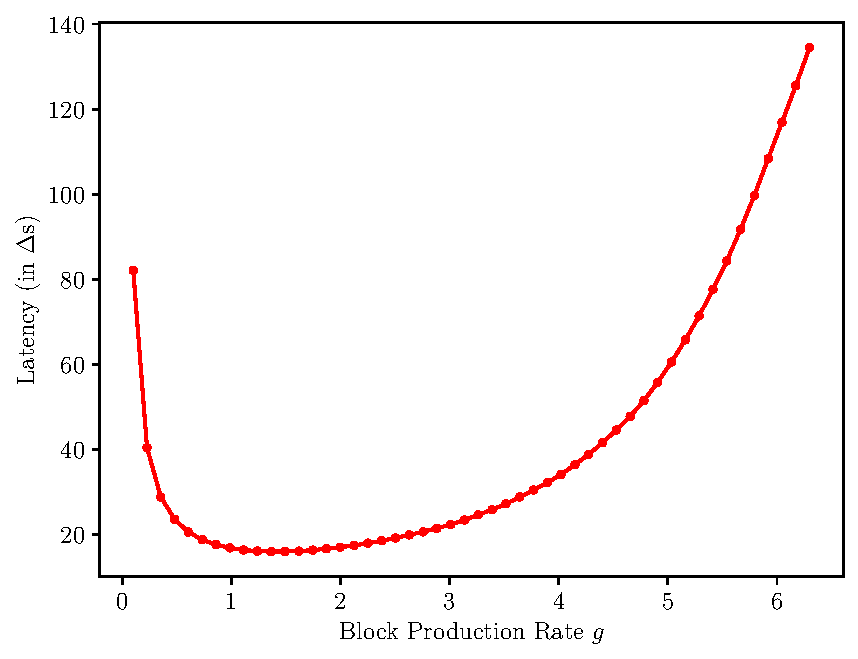
\includegraphics[width = 0.48\textwidth]{figures/g_latency.pdf}

  \caption{Fixing $\beta=0.2$ and $\gamma=0$, we plot the latency of PoEM parameterized under different block production rates $g$.
          For small block production rates, close to zero, we get high latency because blocks are produced very slowly.
          For large block production rates, we get high latency because honest blocks effect many forks, whereas the adversarial blocks
          are all chained in series. We get optimal latency somewhere in the middle.
          The results were obtained by running 100k simulations per point.}
    \label{fig:g_latency}
\end{figure}

We note some limitations of our experimental methodology. Firstly, the private attack has been proven optimal
for Bitcoin only, and not for PoEM, but in our experiments we have used the same attack for both protocols.
Secondly, the optimality of the private attack previously proven~\cite{eiar} is a reduction illustrating
that, for a given resilience $\beta$, if the private attack is not possible, then no attack is possible.
In our experiments, we obtain a safe confirmation parameter $k$ against the private mining attack,
but this confirmation parameter has not been shown to be safe against other attacks, even though the private
mining attack is optimal when it pertains to resilience.
Lastly, there is a discrepancy between the continuous-time model used in our experimental simulations
and the discrete-time model used in our theoretical analysis.

\noindent
\textbf{Real-world Deployment.}
In addition to the above simulations,
we have implemented and deployed\ifanonymous\else\footnote{
    \ifanonymous
        % TODO: add anonymous link here and remove anonymous guard
        The source code will be made available in the full version of this paper.
    \else
        The source code can be found at
        \url{https://github.com/dominant-strategies/go-quai/releases/tag/v0.28.2}
    \fi
}\fi PoEM in a real-world permissionless peer-to-peer
setting.
The deployment is on a testnet that has been continuously operating for
four months. During this period, the network generated 7.5 million blocks
and 500 million transactions
with participation from 2000 miners from the community, maintaining an
average hash rate of 50GH/s using ProgPoW~\cite{progpow}.
The miners computed 518 petahashes in 4 months,
with the difficulty ($\frac{2^{256}}{T}$)
varying between 18 billion and 790 billion.
